\documentclass[12pt]{article}

\usepackage{amsmath,amssymb}
\usepackage{graphicx}

\usepackage{setspace}
\onehalfspacing
\usepackage[margin=1in]{geometry}
\usepackage{hyperref}
\hypersetup{allcolors=blue, colorlinks=true}
\usepackage[utf8]{inputenc}
% Notation
% Mathematical functions
\newcommand{\isone}[1]{{\boldsymbol{1}\left( #1 \right)}}
\renewcommand{\Pr}[1]{{\mathbb{P}\left(#1\right) }}
\newcommand{\f}[1]{{f\left(#1\right) }}
\newcommand{\Prcond}[2]{{\mbox{Pr}\left(#1\vphantom{#2}\;\right|\left.\vphantom{#1}#2\right)}}
\newcommand{\fcond}[2]{{f\left(#1|#2\right) }}
\newcommand{\Expected}[1]{{\mathbb{E}\left\{#1\right\}}}
\newcommand{\ExpectedCond}[2]{{\mathbb{E}\left\{#1\vphantom{#2}\;\right|\left.\vphantom{#1}#2\right\}}}

\newcommand{\Likelihood}[2]{\text{L}\left(#1 \left|\vphantom{#1}#2\right.\right)}
\newcommand{\sufstats}[1]{s\left(#1\right)}
\renewcommand{\exp}[1]{\mbox{exp}\left\{#1\right\}}
\newcommand{\transpose}[1]{{#1}^\mathbf{t}}

% Objects
\newcommand{\params}{\theta}
\newcommand{\Params}{\Theta}
\newcommand{\Graph}{\mathbf{G}}
\newcommand{\graph}{\mathbf{g}}
\newcommand{\GRAPH}{\mathcal{G}}
\newcommand{\Adjmat}{Y}
\newcommand{\adjmat}{y}
\newcommand{\ADJMAT}{\mathcal{Y}}

\newcommand{\INDEPVAR}{\mathcal{X}}
\newcommand{\Indepvar}{X}
\newcommand{\indepvar}{x}

\newcommand{\normconst}{\kappa\left(\params, \Indepvar\right)}

% \graphicspath{{./fig/}}


%% NEED THIS FOR CANCY TEX
\usepackage{pstricks}

% Colors
\definecolor{USCCardinal}{HTML}{990000} % 153 0 0 in RGB
\definecolor{USCGold}{HTML}{FFCC00}
\definecolor{USCGray}{HTML}{CCCCCC}

% To use the function \sout
\usepackage{ulem}
\usepackage{tabularx, booktabs}

% \bibliography{bibliography.bib}

\usepackage{textcomp} % FOR USING THE COPYRIGHT SYMBOL

\title{Exponential Random Graph models for Little Networks\footnote{The authors would like to thank Garry Robins, Carter Butts, Johan Koskinen, Noshir Contractor, and Andrew Slaughter for their valuable contributions to this work. The usual disclaimer applies.\textcopyright{} 2019. This work is licensed under a Creative Commons Attribution-NonCommercial-NoDerivatives 4.0 International License.}}
\author{George G. Vega Yon\footnote{Corresponding author. email: \href{mailto:vegayon@usc.edu}{vegayon@usc.edu}} \and Kayla de la Haye}
\date{Department of Preventive Medicine\\University of Southern California\\ April 2019}

\begin{document}

\maketitle


\section{Introduction}

Statistical models for social networks have enabled researchers to study complex social phenomena that give rise to observed patterns of relationships among social actors, and to gain a rich understanding of the \textit{interdependent nature} of social ties and social actors \cite{Snijders2011,lusher2012exponential}. For example, this research has provided new insights into the role that attributes of social actors (e.g., their characteristics, beliefs, and decisions), and endogenous structural processes (e.g., social balance, and relationship reciprocity) play in shaping social networks in many different populations and social settings, and the influence that these social networks have, in turn, on individuals and groups. 

Much of this research has focused on social networks within medium to large social groups: from a couple of dozen students in a classroom, or colleagues in an organization; to larger social networks within schools, villages, and (online and offline) communities. To date, these advances in statistical models for social networks have rarely been applied to the study of small networks, despite small network data in teams, families, and personal (ego-centric) networks being common in many fields that study social phenomena. The study of small networks often uses descriptive statistics that summarize the structural features of the network; for example, the density, degree distribution, or triad count. However, researchers in these fields are often interested in testing hypotheses about \textit{why} small, localized social structures, such as reciprocity and balance, emerge in these small groups. A key limitation to this work has been the availability of statistical models for networks that can adequately test these hypotheses using an approach that is suited to the dependencies inherent in network data. In this paper, we propose an approach for applying one of the most widely used statistical models for social networks--exponential random graph models, or ERGM--to small graphs, to enable novel and rich research on ``little networks''. 



\def\fig1width{.45\linewidth}
\begin{figure}[tb]
\centering
\begin{tabular}{m{.2\linewidth}<\centering m{.4\linewidth}<\raggedright}
\toprule Representation & Description  \\ \midrule

\includegraphics[width=\fig1width]{mutual.pdf} & Mutual Ties (Reciprocity)\linebreak[4]$\sum_{i\neq j}y_{ij}y_{ji}$  \\
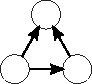
\includegraphics[width=\fig1width]{ttriad.pdf} & Transitive Triad (Balance)\linebreak[4]$\sum_{i\neq j\neq k}y_{ij}y_{jk}y_{ik}$  \\

\includegraphics[width=\fig1width]{homophily.pdf} & Homophily\linebreak[4]$\sum_{i\neq j}y_{ij}\mathbf{1}\left(x_i=x_j\right)$ \\
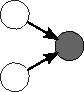
\includegraphics[width=\fig1width]{nodeicov.pdf} & Covariate Effect for Incoming Ties\linebreak[4]$\sum_{i\neq j}y_{ij}x_j$ \\
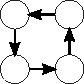
\includegraphics[width=\fig1width]{fourcycle.pdf} & Four Cycle\linebreak[4]$\sum_{i\neq j \neq k \neq l}y_{ij}y_{jk}y_{kl}y_{li}$  \\
\bottomrule
\end{tabular}
\caption{\label{fig:ergm-structs}Besides of the common edge count statistic (number of ties in a graph), ERGMs allow measuring other more complex structures that can be captured as sufficient statistics. }
\end{figure}

\section{Exponential-Family Random Graph Models}

Exponential-Family Random Graph Models (ERGMs) are one of the most popular tools used by social scientists to understand social networks  \cite[and others]{Robins2007,Holland1981,Wasserman1996,Snijders2006}. In this family of models, an observed graph $\adjmat$, or more commonly put, its adjacency matrix representation, is characterized by a set of sufficient statistics, which we denote $\sufstats{}$, as follows:

\begin{equation}
\label{eq:ergm}
  \Prcond{\Adjmat = \adjmat}{\params, \Indepvar} = \frac{%
  	\exp{\transpose{\params}\sufstats{\adjmat, \Indepvar}}%	
  }{
  	\kappa\left(\params, \Indepvar\right)
  },\quad\forall \adjmat\in\ADJMAT
\end{equation}

\noindent Where $\normconst{} = \sum_{\adjmat\in\ADJMAT}\exp{\transpose{\theta}\sufstats{\adjmat, \Indepvar}}$ is the normalizing constant, and $\ADJMAT$ is the support of the model which is usually assumed to include all directed graphs of the same size as $\adjmat$, that are directed, and do not include self-ties. In this case, the size of $\ADJMAT$ equals $2^{n(n-1)}$ possible graphs. This makes the exact calculation of $\normconst{}$, and therfore of \eqref{eq:ergm}, extremely complicated to calculate. \autoref{fig:ergm-structs} shows some examples on structures (statistics) that can be used with ERGMs.

Modeling ``small networks'' is a topic mentioned several times in the literature on social network models  \cite{Wasserman1996,Frank1986,Snijders2011},  although much less frequently than studies of large networks, and applications of network models such as ERGMs to small networks are rare.\footnote{Perhaps because that, as put by \cite{Snijders2011}, small networks are considered to be ``uninteresting special cases''} Thus, ERGM methods have been developed to accommodate larger networks (although they do not scale well to ``very large'' networks of several thousand nodes or more). For example, rather than calculating the likelihood function using exhaustive enumeration (which we will refer as exact likelihood), the most popular software packages used for estimating these models apply simulation-based estimation methods.

As a consequence, the methods used to estimate ERGMs for large networks do not translate well to small network data (i.e., 10 or fewer nodes). The inference degeneracy problem--which arises when parameter estimation depends on Monte Carlo quadrature \cite{Handcock2003}--often encountered with these methods, even with large networks, is even more prevalent in the case of small networks. For example, if we are trying to estimate an ERGM in a network with only three nodes, in the scenario where the graph is directed and does not allow for self-ties, the chances of obtaining a graph with 1 or zero ties (emtpy or almost completely empty), or one with 5 or 6 ties (fully or almost fully connected) is about 20\% using a uniform sampler. The degeneracy problem is so common with small networks (e.g., 3 to 10 nodes) that practitioners typically cannot estimate ERGMs for small graphs. One work-around that is sometime attempted when multiple small networks are observed, is to aggregate the small networks into one large graph to obtain something similar to pooled estimates. Specifically, practitioners stack multiple adjacency matrices as a single matrix  building a block-diagonal data set, explicitly modeling the networks as independent by fixing the ``off diagonal'' components to 'impossible' (i.e., structural zeros). The problem with this approach is that the very set of constraints that are subscribed to the model make the sampling procedure complicated. 

To overcome this issue, we leverage the fact that in the case of small networks the likelihood function is tractable, and therefore we can directly estimate model parameters without using Markov Chain Monte Carlo (MCMC) methods, avoiding the convergence issues associated with inference degeneracy \cite{Handcock2003}. In this paper, we revisit ERGMs for small networks, which we define as those networks in which enumerating the entire support of the distribution is possible using modern computers (i.e., networks of size 3 to 6 nodes). We propose an estimation process that can be used in this type of application, and present results from an extensive simulation study evaluating the feasibility and validity of this method.

\section{\ergmitos{}: ERGMs for small networks}

With modern computers, calculating the exact likelihood function of an ERGM for a small network becomes computationally feasible. This has an important implication: the process for estimating the parameters of an ERGM for small networks can be done directly, rather than having to use simulation-based methods that are required when fitting ERGMs to larger networks. This exact calculation would not only obtain a better solution (in general) compared to simulation methods, but also, if the MLEs exists, it can help to mitigate the degeneracy problem. Although the degeneracy problem is not completely avoided, it is important to note that this approach will reach a better situation compared to MC-MLE estimation. As stated by \cite[p. 7]{Handcock2003}: "[i]f the model used to simulate the graphs is not close enough to produce realizations that cover the observed values of the statistics, the MC-MLE will not exist even in cases where the MLE does." In other words, the non-existence of MC-MLE estimates does not imply the non-existence of MLE estimates.

Small network data is typically collected from \textit{samples} of groups, so that multiple networks are observed from a sample of, for example, families, small teams, or ego-networks. This type of study design often allows us to assume that we have observed multiple independent networks, and that the data generating process is shared across the sampled networks. If we can adopt both of these assumptions, a pooled model can be estimated by maximizing the following joint-likelihood:

\begin{equation}
    \label{eq:ergm-pooled}
    \Prcond{\Adjmat_1 = \adjmat_1, \dots, \Adjmat_P = \adjmat_P}{\params, \Indepvar_1, \dots, \Indepvar_p} = \prod_{p=1}^P\frac{%
    		\exp{\transpose{\params}\sufstats{\adjmat_p, \Indepvar_p}}%	
    	}{
    		\kappa_p\left(\params, \Indepvar_p\right)
    	}
\end{equation}

\noindent Where $P$ denotes the number of networks used in the model. We call this framework, which is just a revisited version of ERGM in the case of small networks, \ergmito{}\footnote{The \textit{ito}/\textit{ita} suffix is used in Spanish to denote small, or affection. We are particularly grateful to George Barnett who proposed the name during the North American Social Networks Conference on 2018.}.

One potential problem that we are not addressing with the pooled estimates is the problem of scalability, and in particular the interpretation of the constant parameter in the model; the edge count parameter. In the baseline case of estimating a density parameter using a single network, as pointed out in \cite{Krivitsky2011}, extrapolating or comparing that estimate in the context of a network with a different sizes may be complicated in the sense that, if left as is, a fixed density parameter assumes a constant change in the average degree of the network, which may not be realistic in some scenarios. Instead it may be more natural to think that the degree holds constant. This, in the case of pooled ERGMs, poses a problem in terms of assuming that the networks included in the model share a common data-generating-process, and thus, the same edge count or density parameter. Notwithstanding this is an important problem to consider when dealing with networks of different sizes, the cases pointed out by \cite{Krivitsky2011} discuss situations in which the sizes of the networks range from a few dozens to a couple of thousands, which is not the case here.

The simulations and model fitting were conducted using the R package \texttt{ergmito} which has been developed to implement the methods described in this work.

\section{Illustration with simulated data: fivenets}

\subsection{Data-generating-process and model fitting}

In the following section we work with a simulated data set that was created using the data-generating-process of \ergmitos{}. This particular dataset, which we call ``fivenets'', is included in the in the R package \texttt{ergmito}\footnote{The R package is available to be downloaded at  \url{https://github.com/muriteams/ergmito}.}. The data set contains five simulated networks with nodal attributes (we use gender in the following example), and the networks were generated using the following specification:

\begin{multline*}
\Prcond{\Adjmat = \adjmat}{\Indepvar_{\mbox{gender}}, \params} = \\
\frac{ %
    \exp{\params_{edges}\left(\sum_{i,j} \adjmat_{ij}\right) + %
    \params_{homophily}\left(\sum_{i,j} \adjmat_{ij}\isone{\Indepvar_{gender, i} = \Indepvar_{gender, j}}}\right) %
    }{%
    \normconst{}
    }
\end{multline*}

\noindent where $\params_{edges} = -2.0$ and $\params_{homophily} = 2$. Using this equation we draw five networks of size five. The process of ``homophily'' is represented by a parameter that is defined as the number of ties in which ego and alter have the same gender. Before drawing the networks we randomly generated the node attribute (gender) parameter to each vertex as a Bernoulli with parameter 0.5. \autoref{fig:fivenets} shows the generated networks, including their nodal attributes.

\begin{figure}[tb]
    \centering
    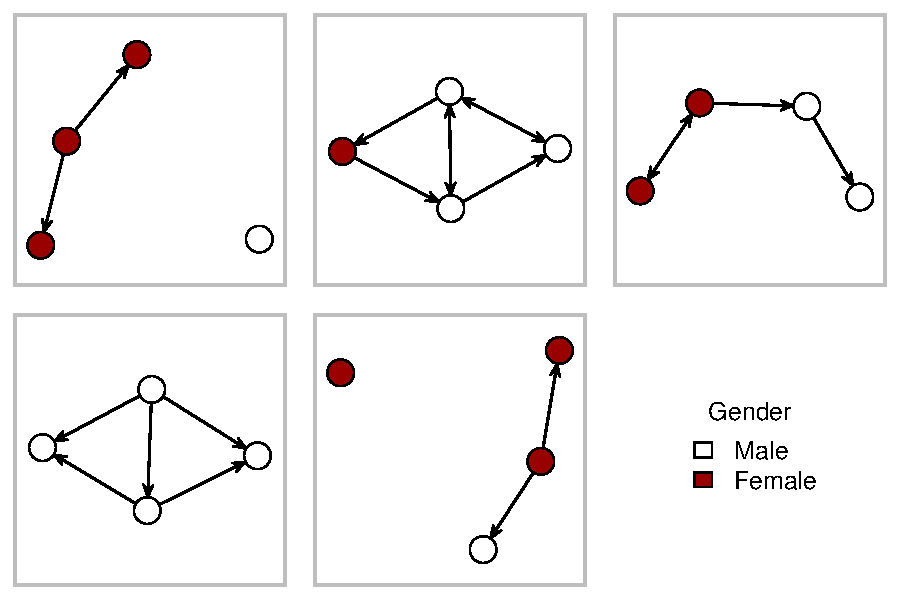
\includegraphics[width=.6\linewidth]{fivenets_graphs.pdf}
    \caption{\label{fig:fivenets}Fivenets data set. These graphs were randomly drawn from an ERGM distribution with two parameters: number of edges and gender homophily, with parameters equal to -2.0 and 2.0 respectively.}
    \label{fig:my_label}
\end{figure}

Using the \texttt{ergmito} R package, we fit three different models to the data\footnote{Some details regarding the computational aspects of the model fitting process are provided in \ref{appendix:mle}.}: (1) a Bernoulli graph, which is a model that only includes the ``edges'' parameter, (2) a model with ``gender homophily" as its only parameter, and finally (3) a model including both ``edges'' and ``gender homophily'', this is, the correct specification of the model. \autoref{table:coefficients} shows the estimation results of the three different specifications of the model and as expected, model (3) has the best overall fit to the data. The \textit{goodness of fit} of this model is evaluated in the following section.


\begin{table}
\begin{center}
\begin{tabular}{l c c c }
\hline
 & Homopholy & Edgecount & Full model \\
\hline
Edgecount             &          & $-0.69^{*}$ & $-1.70^{**}$ \\
                      &          & $(0.27)$    & $(0.54)$     \\
Homophily (on Gender) & $-0.12$  &             & $1.59^{*}$   \\
                      & $(0.34)$ &             & $(0.64)$     \\
\hline
AIC                   & 85.06    & 78.38       & 73.34        \\
BIC                   & 87.15    & 80.48       & 77.53        \\
Log Likelihood        & -41.53   & -38.19      & -34.67       \\
Num. networks         & 5        & 5           & 5            \\
\hline
\multicolumn{4}{l}{\scriptsize{$^{***}p<0.001$, $^{**}p<0.01$, $^*p<0.05$}}
\end{tabular}
\caption{Fitted ERGMitos using the fivenets dataset. As expected, the Full model (last column of the table) has overall a better fit of the data. More over, the 95\% level CI of each covers the true parameters: $\hat\theta_{edges} \in [-2.77, -0.64]$; $\hat\theta_{Homophily} \in [0.33, 2.85]$.}
\label{table:coefficients}
\end{center}
\end{table}


\subsection{Goodness-of-fit in \ergmitos}

Researchers that apply ERGMs should be familiar with the goodness-of-fit (GOF) diagnostics that are used to assess how well the estimated model can reproduce graphs that are similar to the observed graph on a range of local and global graph statistics. One of the statistics that is often scrutinized in these analyses, because of the difficulty in obtaining a good fit, is the distribution of shortest-path lengths (or geodesic distribution). In the case of \ergmitos{} this global statistic is clearly less relevant because the shortest-path lengths between any two nodes in a small network typically lies between 1 and 2 steps. Therefore, we focus our GOF analysis on the parameters fit in the model as the bare-minimum of local graph statistics, as shown in \autoref{fig:fivenets-gof}. An important difference in our approach compared to traditional GOF assessments for ERGMs is that we are able to enumerate the full support of the model, and so instead of evaluating a boxplot we present a 90\% exact confidence interval per-statistic per network, comparing the fitted model's distribution with the observed parameters. A detailed discussion of this aspect of the \ergmitos{} is presented at the end of this paper.

\begin{figure}[tb]
    \centering
    \caption{Goodness-of-fit in \ergmitos{}. In this case we are showing how do the observed sufficient statistics of each one of the 5 networks (x-axis) locate in the overall estimated distribution based on the fitted \ergmito{}. The gray lines in each box show the minimum and maximum value that the sufficient statistics can take in each one of the 5 networks, whereas the dotted lines provide a 90\% confidence interval. The dots are the observed statistics in each network.}
    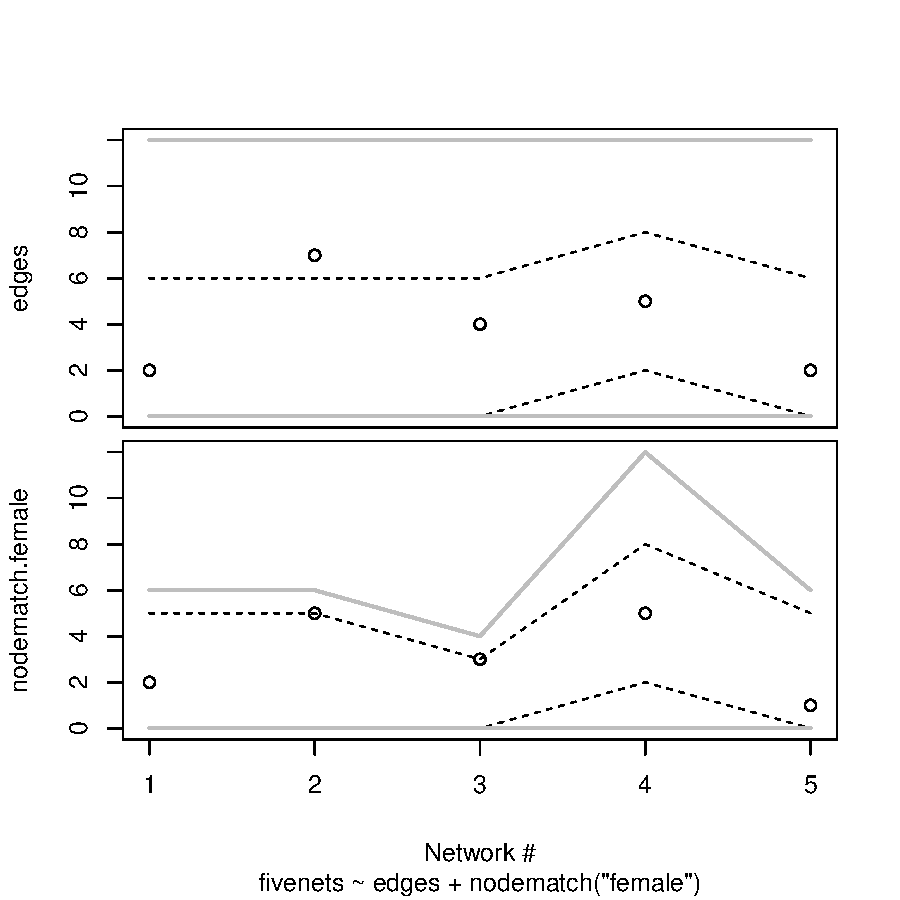
\includegraphics[width=.7\linewidth]{fivenets_gof.pdf}
    \label{fig:fivenets-gof}
\end{figure}

An important advantage of the \ergmitos{} over ``regular'' ERGMs is that we can observe the surface of the log-likelihood over different combinations of parameters in a rather straightforward way. This, together with the GOF analysis should be a routine step done after every \ergmito{} fit. \autoref{fig:fivenets-loglike} shows the surface of the log-likelihood function around the solution parameters to the maximization problem.

\begin{figure}[tb]
    \centering
    \caption{Surface of the log-likelihood function of the pooled \ergmito{} model. Lighter colors represent higher values while darker ones represent lower values. The red dot corresponds to the location of the MLE estimate of the model.}
    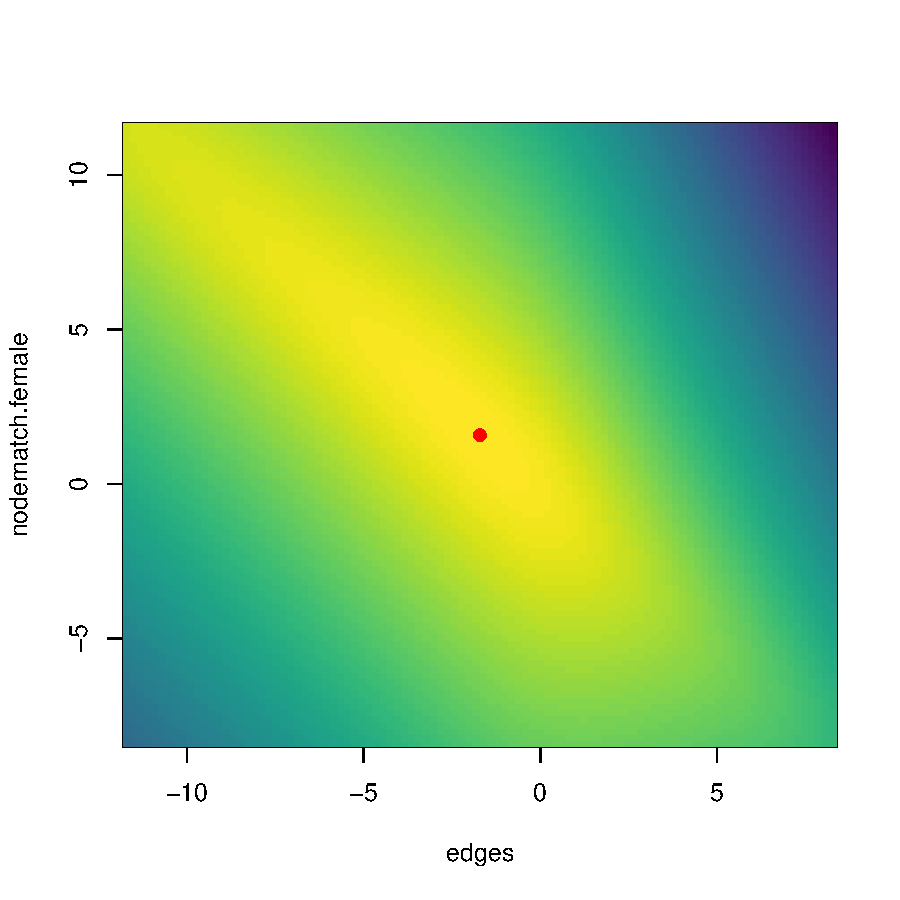
\includegraphics[width=.7\linewidth]{fivenets_loglike.pdf}
    \label{fig:fivenets-loglike}
\end{figure}

Being able to calculate the surface of the exact likelihood function in a rather (computationally) trivial way, allows us to assess quite easily the quality of the estimated set of parameters. One good use of this diagnostic is to evaluate the roughness of the log-likelihood function, which in principle should give us an idea of the likelihood of the maximization process failing to reach a global maxima.

\pagebreak
\section{Simulation study}

\subsection{Sampling groups of small networks}

We conducted a simulation study to explore the properties of MLE for small networks. Using the \texttt{ergmito} R package, we generated 100,000 samples of groups of small networks, each one with an average of 30 networks, resulting in approximately 3 million small networks drawn from an ERGM distribution. Specifically, to generate each one of the 100,000 samples we did the following:

\begin{enumerate}

\item Draw two numbers from a piece-wise Uniform with values in $[-4, -.1]\cup[.1, 4]$, which corresponded to the parameters \textbf{edgecount} ($\params_{edges}$) and number of \textbf{mutual ties} ($\params_{mutuality}$) for the sufficient statistics.\footnote{This is akin to \cite{Schweinberger2015} approach to simulate ERGM from outside of degenerate areas, although we take a more conservative approach than their ranges of (-5,0) and (0, 5) for the parameters ``edges'' and ``triangles''. We removed some samples in which the model was not able to be fit due to near-degenerate structures.}

\item The number of networks included in the sample was obtained from 3 Poisson distributions with the parameter mean equal to 10, in particular, each one of those specified how many networks of sizes 3 ($n_3$), 4 ($n_4$), and 5 ($n_5$) would be generated. This implies that on average each sample has ten networks of each size, this is, a total of 30 networks per sample.

\item Finally we draw $n_3$, $n_4$, and $n_5$ networks of sizes 3, 4, and 5 respectively from ERGM distributions with parameters $(\params_{edges}, \params_{mutuality})$ (so all 3 network sizes share the same set of population parameters). We then repeated step 1 through 3 100,000 times.
\end{enumerate}

Unfortunately, given the small size of these networks, it is easy to simulate population parameters that fell within the almost-degenerate (and actually, degenerate) region of the parameter space. Because of this reason, the final analysis only considers 54,995 samples since the reminder set of samples were not informative as those were composed either of (nearly-)fully connected or (nearly-)fully empty graphs. The next section discusses the results.

\subsection{Results}

As shown in \autoref{fig:bias}, the model appears to behave well, in general, in terms of empirical bias. While we observe some cases in which the estimates are significantly biased (in either direction), most of the distribution falls within the $[-1,1]$ region.

\begin{figure}
	\centering
	\caption{\label{fig:power}Empirical power by sample size and model parameter.}
	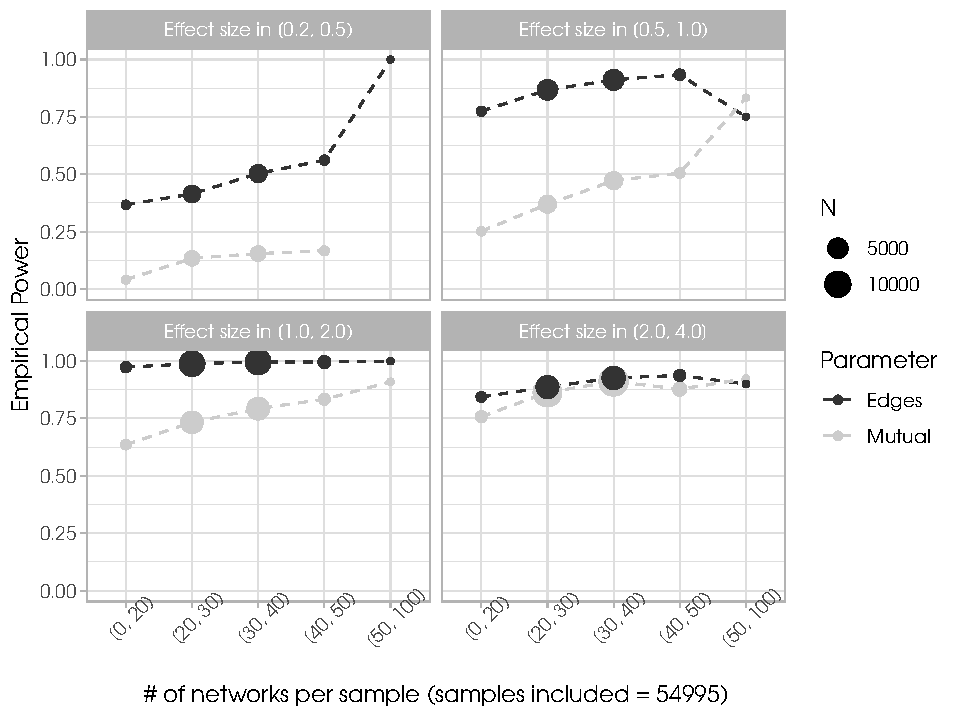
\includegraphics[width=.9\linewidth]{power-02-various-sizes-3-5.pdf}
\end{figure}

Another feature that was important to evaluate was power. \autoref{fig:power} shows the empirical power level achieved at various sample sizes for the two parameters. Overall, we observe that, as expected, the empirical power grows as the sample sizes increases. The few exceptions to this that can be observed in the figures are due to insufficient samples simulated for the cases where there 50 or more networks per sample (for example), which were significantly fewer observations compared to, for example, those which had between 20 to 40 networks (recall that the expected sample size in this simulation study is 30 networks per sample).

It is interesting to notice that in the case of effect sizes of magnitude [1.0, 2.0) the discovery rate for the `Mutual` parameter reaches around 0.75 for sample sizes between 30 to 40 networks, which is a rather common sample size in the study of small networks such as teams, ego-networks or families.

\begin{figure}
    \centering
    \caption{\label{fig:bias}Violin plots showing the empirical distribution of the bias per model parameter. In general we see that the parameter estimates' bias is centered around zero and in all but a few cases within the range [-1, 1]. Just like the figure on empirical power, this figure contains 54,995 samples.}
    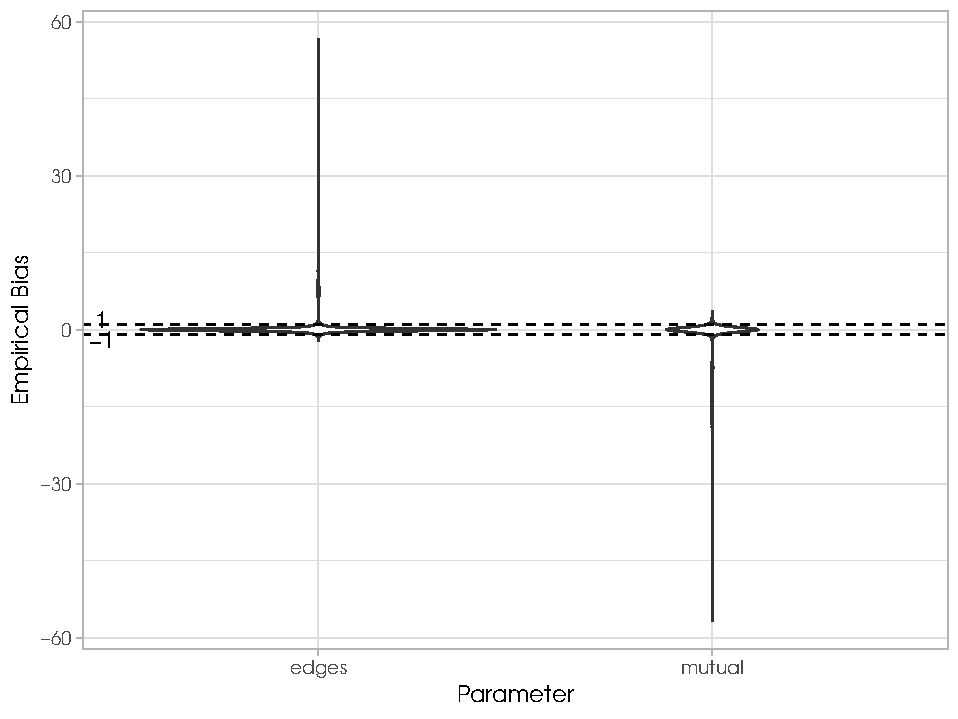
\includegraphics[width=.8\linewidth]{bias-02-various-sizes-3-5.pdf}
\end{figure}

The code used to reproduce this entire section can be found at \url{https://github.com/muriteams/ergmito-simulations}.

\pagebreak
\section{Discussion}

In this paper revisit the Exponential Family Random Graph Models (ERGM) for the case of small networks. In response to approaches for modeling small networks having been overlooked in the literature, we propose ERGMs for small networks, or \ergmitos{} as we call them. These models have the nice feature that they can be estimated using Maximum Likelihood Estimation directly without having to recur to estimation via MCMC methods, as is traditionally done with ERGM for larger networks. This approach provides several benefits for small network data, mainly: (1) we avoid at least partially, if not completely, the model near-degeneracy problems that affects the aforementioned methods; and (2) given the natural prevalence of samples of small networks like multiple families, small teams, or ego networks, pooling estimates are a natural application for small network data. We find that  we are able to estimate such models easily, and that this approach improves accuracy and efficiency for modeling small networks.

Unanswered questions that will be a topic for future work include how to analyze \ergmitos{}. More work is needed on how to evaluate goodness-of-fit, and identify the statistics that are most important to evaluate and that are reasonable to expect in a model that would suggest a ``good fit''. A feature of  \ergmitos{} that is in our favor to facilitate this future work is that they enable a rather simple way of conducting simulation studies (relative to traditional ERGMs).

Overall,  \ergmitos{} provide a promising extension to the ERGM framework for the analysis of small social networks, which can generate a richer understanding of the local social processes that give rise to the formation of networks in small social groups. 

\section{Acknowledgements}

This material is based upon work support by, or in part by, the U.S. Army Research Laboratory and the U.S. Army Research Office under grant number W911NF-15-1-0577. The views, opinions, and/or findings contained in this paper are those of the authors and shall not be construed as an official Department of the Army position, policy, or decision, unless so designated by other documents

Computation for the work described in this paper was supported by the University of Southern California’s Center for High-Performance Computing (hpcc.usc.edu).

\clearpage

\bibliographystyle{plain}
\nocite{vegayon2019,R,butts2016,Wickham2016,Leifeld2013}
\bibliography{bibliography.bib}

\clearpage

\appendix

\section{MLE\label{appendix:mle}}

The estimation process of \ergmitos{} (as pooled models of small networks) is done entirely on R using the \texttt{ergmito} R package. While a significant amount of the implementation of the methods described here was done using \texttt{Rcpp} \cite{Eddelbuettel2011}, a core component of the package is based on statnet's \texttt{ergm} R package, and in particular, in the function \texttt{ergm.allstats} which does exhaustive enumeration of statistics in a compact way. In general, the estimation process for any list of networks is as follows:

\begin{enumerate}
    \item Analyze the model to be estimated, this is, extract the networks from the left-hand-side as specified in the ergm package, and calculate the exact statistics using the ergm.allstats function.
    \item With the full enumeration of statistics, write down the joint likelihood function of the model in a compact form, this is, using the weights instead of the full enumeration of the support of the model. Overall this helps with speed when it comes to evaluate the log-likelihood function.
    \item Since we are dealing with exact statistics, it is also possible to calculate the exact gradient function. We compute the gradient as follows:
    
    \begin{equation}
    \sum_{p}\nabla l_p(\theta) = \transpose{\sufstats{\adjmat_p, \Indepvar_p}} - \frac{\transpose{Q_p}\left(\transpose{W_p} \circ \exp{Q_p \theta}\right)}{\kappa_p}
    \end{equation}
    
    Where $\sufstats{\adjmat, \Indepvar}$ is a vector of observed sufficient statistics (usually called target statistics), $Q$ is a matrix of sufficient statistics, in particular, the isomorphic sufficient statistics associated with the model, and $W$ is a vector of frequency weights.
    
    \item With the previous steps as the part of the algorithm that takes the most time, we then maximize the joint-log-likelihood using the optim function in the R stats, and in particular, the BFGS algorithm for quasi-Newtonian optimization, and we do this several times (right now, the default option asks the optimization to be done 5 times), everytime starting from a different point in the parameter space.
    
    \item Finally, we keep the set of parameters that reached the highest value for the joint-log-likelihood function.
\end{enumerate}



\end{document}
